\section{Iterative Deepening Search (IDS) \cite{ai/book/Artificial-Intelligence-A-Modern-Approach/Russell-Norvig}}
\label{AI: Algorithms/Iterative Deepening Search (IDS)}


\begin{figure}[h!]
    \centering
    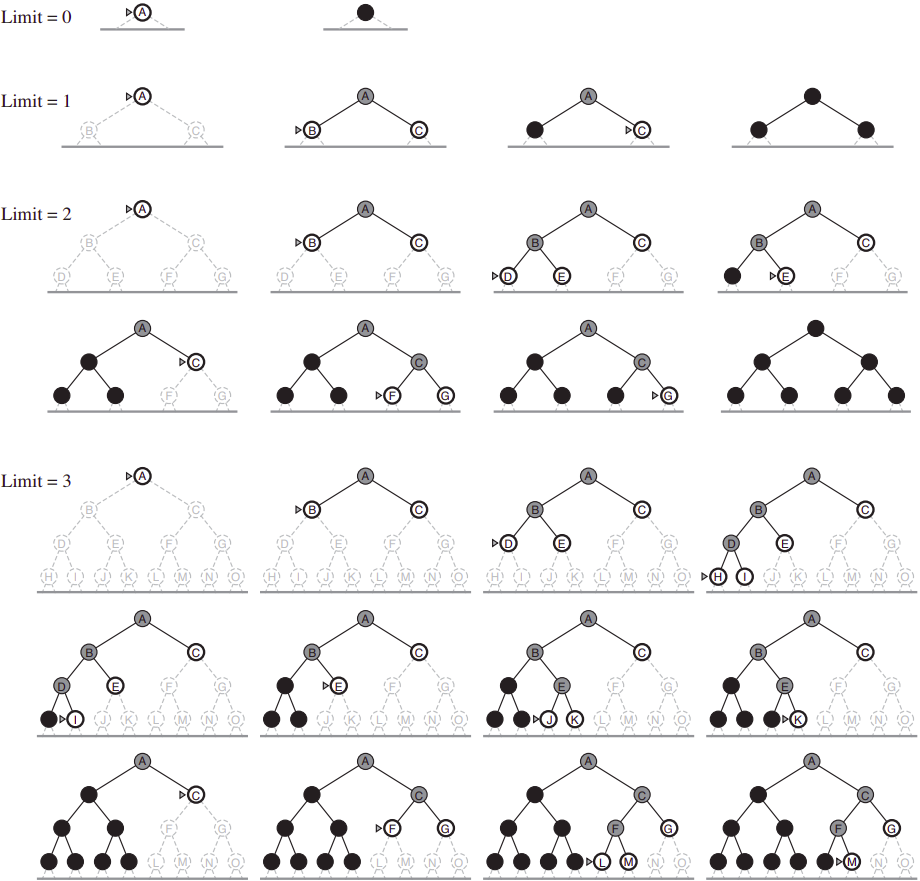
\includegraphics[
        width=\linewidth,
        height=14cm,
        keepaspectratio,
    ]{images/algorithms/iterative-deepening-search-BT.png}
    \caption*{Four iterations of iterative deepening search on a binary tree \cite{ai/book/Artificial-Intelligence-A-Modern-Approach/Russell-Norvig}}
\end{figure}


\begin{enumerate}[itemsep=0.2cm]
    \item \textbf{Iterative deepening search} (or \textbf{iterative deepening depth-first search}) is a general strategy, often used in combination with depth-first tree search, that finds the best depth limit.
    \hfill \cite{ai/book/Artificial-Intelligence-A-Modern-Approach/Russell-Norvig}

    \item It gradually increases the depth limit $\ell \in \dCurlyBrac{0,1,2,\cdots,\infty}$ till a goal is found, which occurs when $\ell = d$ ($d$ is unknown in reality)
    \hfill \cite{ai/book/Artificial-Intelligence-A-Modern-Approach/Russell-Norvig}

    \item Iterative deepening combines the benefits of depth-first and breadth-first search.
    \hfill \cite{ai/book/Artificial-Intelligence-A-Modern-Approach/Russell-Norvig}
    \begin{enumerate}[itemsep=0.2cm]
        \item Like depth-first search, its memory requirements are modest: $\mathcal{O}(b d)$ to be precise. 
        \hfill \cite{ai/book/Artificial-Intelligence-A-Modern-Approach/Russell-Norvig}

        \item Like breadth-first search, it is complete when the branching factor is finite and optimal when the path cost is a non-decreasing function of the depth of the node.
        \hfill \cite{ai/book/Artificial-Intelligence-A-Modern-Approach/Russell-Norvig}
    \end{enumerate}

    \item total number of nodes generated in the worst case is
    \\
    $N(\text{IDS})=(d)b + (d - 1)b^2 + \cdots + (1)b^d$
    \hfill \cite{ai/book/Artificial-Intelligence-A-Modern-Approach/Russell-Norvig}

    \item you can use a hybrid approach that runs breadth-first search until almost all the available memory is consumed, and then runs iterative deepening from all the nodes in the frontier.
    \hfill \cite{ai/book/Artificial-Intelligence-A-Modern-Approach/Russell-Norvig}

    \item iterative deepening is the \textit{preferred uninformed search} method when the search space is large and the depth of the solution is not known.
    \hfill \cite{ai/book/Artificial-Intelligence-A-Modern-Approach/Russell-Norvig}

    \item \textbf{Performance}:
    \begin{enumerate}[itemsep=0.2cm]
        \item \textbf{completeness}: YES \textbf{if} $b$ is finite \textbf{else} NO
        \hfill \cite{ai/book/Artificial-Intelligence-A-Modern-Approach/Russell-Norvig}

        \item \textbf{optimal}: YES \textbf{if} path cost is a non-deceasing function of depth of the node \textbf{else} NO
        \hfill \cite{ai/book/Artificial-Intelligence-A-Modern-Approach/Russell-Norvig}
        
        \item \textbf{space complexity}: $\mathcal{O}(b d)$
        \hfill \cite{ai/book/Artificial-Intelligence-A-Modern-Approach/Russell-Norvig}

        \item \textbf{time complexity}: $\mathcal{O}(b^d)$
        \hfill \cite{ai/book/Artificial-Intelligence-A-Modern-Approach/Russell-Norvig}
    \end{enumerate}
\end{enumerate}

\vspace{0.5cm}

\begin{algorithm}[H]
    \caption{The iterative deepening search algorithm, which repeatedly applies depth-limited search with increasing limits. It terminates when a solution is found or if the depth-limited search returns failure, meaning that no solution exists. \cite{ai/book/Artificial-Intelligence-A-Modern-Approach/Russell-Norvig}}

    \SetKwFunction{FUNCTION}{\textsc{Iterative-Deepening-Search}}
    \SetKwProg{Fn}{function}{ returns \normalfont{a solution, or failure}}{end}
    \Fn{\FUNCTION{problem}}{
        \For{\normalfont $depth = 0$ \textbf{to} $\infty$}{
            $result \gets$ \textsc{Depth-Limited-Search}($problem,\ depth$)\\
            \If{$result \neq cutoff$}{
                \Return $result$
            }
        }
    }
\end{algorithm}


\begin{lstlisting}[
    language=Python,
    caption=Problem Solving Agent - Iterative Deepening Search 
]
def iterative_deepening_search(problem: Problem, limit=1000000):
    for i in range(limit):
        result = depth_limited_search(problem, i)
        if result != CUTOFF:
            return result
\end{lstlisting}






